\documentclass{standalone}

\usepackage[OT1]{fontenc}
\renewcommand*\familydefault{\sfdefault}
\usepackage{helvet,sfmath}
\usepackage{siunitx}

\usepackage{tikz}
\usetikzlibrary{arrows,calc,patterns}
\usetikzlibrary{intersections, calc, arrows.meta}
\usepackage{tikz,tkz-euclide}

\begin{document}






\tikzset{every picture/.style={line width=0.75pt}} %set default line width to 0.75pt        

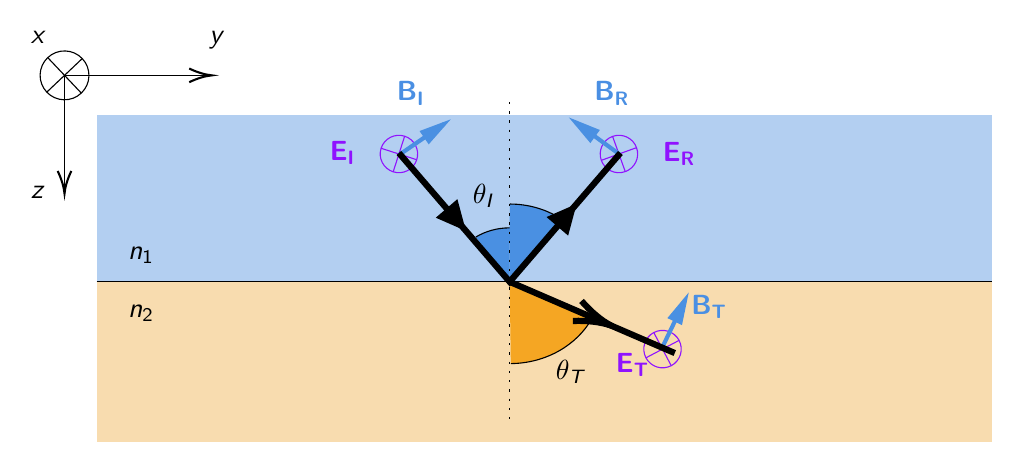
\begin{tikzpicture}[x=0.75pt,y=0.75pt,yscale=-1,xscale=1]
%uncomment if require: \path (0,5487); %set diagram left start at 0, and has height of 5487

%Shape: Rectangle [id:dp6347626919288062] 
\draw  [draw opacity=0][fill={rgb, 255:red, 241; green, 187; blue, 99 }  ,fill opacity=0.51 ] (50,208.16) -- (481.5,208.16) -- (481.5,285.45) -- (50,285.45) -- cycle ;
%Shape: Ellipse [id:dp871868401229967] 
\draw  [color={rgb, 255:red, 144; green, 19; blue, 254 }  ,draw opacity=1 ] (318.39,232.62) .. controls (322.8,230.3) and (328.25,231.99) .. (330.58,236.39) .. controls (332.9,240.8) and (331.21,246.26) .. (326.8,248.58) .. controls (322.4,250.9) and (316.94,249.21) .. (314.62,244.8) .. controls (312.3,240.4) and (313.99,234.94) .. (318.39,232.62) -- cycle ;
%Straight Lines [id:da20088089131792708] 
\draw [color={rgb, 255:red, 144; green, 19; blue, 254 }  ,draw opacity=1 ]   (330.58,236.39) -- (314.62,244.8) ;
%Straight Lines [id:da5797567927305401] 
\draw [color={rgb, 255:red, 144; green, 19; blue, 254 }  ,draw opacity=1 ]   (318.39,232.62) -- (326.8,248.58) ;

%Shape: Rectangle [id:dp21019392123200042] 
\draw  [draw opacity=0][fill={rgb, 255:red, 114; green, 167; blue, 229 }  ,fill opacity=0.54 ] (50,128) -- (481.5,128) -- (481.5,208.16) -- (50,208.16) -- cycle ;
%Shape: Ellipse [id:dp38676189682956585] 
\draw  [color={rgb, 255:red, 144; green, 19; blue, 254 }  ,draw opacity=1 ] (298.54,138.11) .. controls (303.23,136.43) and (308.4,138.86) .. (310.08,143.54) .. controls (311.77,148.23) and (309.34,153.4) .. (304.65,155.08) .. controls (299.97,156.77) and (294.8,154.34) .. (293.11,149.65) .. controls (291.43,144.97) and (293.86,139.8) .. (298.54,138.11) -- cycle ;
%Straight Lines [id:da2704183830735446] 
\draw [color={rgb, 255:red, 144; green, 19; blue, 254 }  ,draw opacity=1 ]   (310.08,143.54) -- (293.11,149.65) ;
%Straight Lines [id:da7069475142095621] 
\draw [color={rgb, 255:red, 144; green, 19; blue, 254 }  ,draw opacity=1 ]   (298.54,138.11) -- (304.65,155.08) ;

%Shape: Ellipse [id:dp3978315670850736] 
\draw  [color={rgb, 255:red, 144; green, 19; blue, 254 }  ,draw opacity=1 ] (187.01,143.83) .. controls (188.54,139.09) and (193.62,136.49) .. (198.36,138.02) .. controls (203.1,139.54) and (205.71,144.63) .. (204.18,149.37) .. controls (202.65,154.11) and (197.57,156.71) .. (192.83,155.18) .. controls (188.09,153.65) and (185.49,148.57) .. (187.01,143.83) -- cycle ;
%Straight Lines [id:da9199787907559669] 
\draw [color={rgb, 255:red, 144; green, 19; blue, 254 }  ,draw opacity=1 ]   (198.36,138.02) -- (192.83,155.18) ;
%Straight Lines [id:da5716396700832854] 
\draw [color={rgb, 255:red, 144; green, 19; blue, 254 }  ,draw opacity=1 ]   (187.01,143.83) -- (204.18,149.37) ;

%Shape: Arc [id:dp29391108225428286] 
\draw  [draw opacity=0][fill={rgb, 255:red, 74; green, 144; blue, 226 }  ,fill opacity=1 ] (232.64,186.6) .. controls (237.3,183.81) and (242.91,182.18) .. (248.95,182.18) .. controls (248.97,182.18) and (248.99,182.18) .. (249.01,182.18) -- (248.95,208.16) -- cycle ; \draw   (232.64,186.6) .. controls (237.3,183.81) and (242.91,182.18) .. (248.95,182.18) .. controls (248.97,182.18) and (248.99,182.18) .. (249.01,182.18) ;  
%Shape: Arc [id:dp6337223162167127] 
\draw  [draw opacity=0][fill={rgb, 255:red, 74; green, 144; blue, 226 }  ,fill opacity=1 ] (249,170.7) .. controls (258.27,170.71) and (266.83,173.37) .. (273.78,177.88) -- (248.95,208.16) -- cycle ; \draw   (249,170.7) .. controls (258.27,170.71) and (266.83,173.37) .. (273.78,177.88) ;  
%Shape: Arc [id:dp5886542657439651] 
\draw  [draw opacity=0][fill={rgb, 255:red, 245; green, 166; blue, 35 }  ,fill opacity=1 ] (288.5,226.04) .. controls (281.24,238.69) and (266.53,247.4) .. (249.52,247.58) -- (248.95,208.16) -- cycle ; \draw   (288.5,226.04) .. controls (281.24,238.69) and (266.53,247.4) .. (249.52,247.58) ;  
%Straight Lines [id:da012823076022556945] 
\draw [color={rgb, 255:red, 74; green, 144; blue, 226 }  ,draw opacity=1 ][line width=1.5]    (195.59,147.1) -- (217.3,132.16) ;
\draw [shift={(220.59,129.89)}, rotate = 145.45] [fill={rgb, 255:red, 74; green, 144; blue, 226 }  ,fill opacity=1 ][line width=0.08]  [draw opacity=0] (15.6,-3.9) -- (0,0) -- (15.6,3.9) -- cycle    ;
%Straight Lines [id:da06657178822561982] 
\draw [color={rgb, 255:red, 74; green, 144; blue, 226 }  ,draw opacity=1 ][line width=1.5]    (301.84,146.71) -- (280.73,131.35) ;
\draw [shift={(277.5,129)}, rotate = 36.05] [fill={rgb, 255:red, 74; green, 144; blue, 226 }  ,fill opacity=1 ][line width=0.08]  [draw opacity=0] (15.6,-3.9) -- (0,0) -- (15.6,3.9) -- cycle    ;
%Straight Lines [id:da3924264901753851] 
\draw [color={rgb, 255:red, 74; green, 144; blue, 226 }  ,draw opacity=1 ][line width=1.5]    (322.23,240.3) -- (333.49,216.9) ;
\draw [shift={(335.23,213.3)}, rotate = 115.71] [fill={rgb, 255:red, 74; green, 144; blue, 226 }  ,fill opacity=1 ][line width=0.08]  [draw opacity=0] (15.6,-3.9) -- (0,0) -- (15.6,3.9) -- cycle    ;
%Straight Lines [id:da4144667492198211] 
\draw    (50,208.16) -- (481.5,208.16) ;
%Straight Lines [id:da5725620473171738] 
\draw  [dash pattern={on 0.84pt off 2.51pt}]  (248.95,121.51) -- (248.95,276.08) ;
%Straight Lines [id:da5692190223883713] 
\draw [line width=2.25]    (195.59,146.1) -- (248.95,208.16) -- (302.31,146.1) ;
\draw [shift={(227.88,183.65)}, rotate = 229.31] [fill={rgb, 255:red, 0; green, 0; blue, 0 }  ][line width=0.08]  [draw opacity=0] (14.29,-6.86) -- (0,0) -- (14.29,6.86) -- cycle    ;
\draw [shift={(281.24,170.61)}, rotate = 130.69] [fill={rgb, 255:red, 0; green, 0; blue, 0 }  ][line width=0.08]  [draw opacity=0] (14.29,-6.86) -- (0,0) -- (14.29,6.86) -- cycle    ;
%Straight Lines [id:da009432972183710864] 
\draw [line width=2.25]    (248.95,208.16) -- (328.5,242.5) ;
\draw [shift={(297.54,229.14)}, rotate = 203.35] [color={rgb, 255:red, 0; green, 0; blue, 0 }  ][line width=2.25]    (17.49,-5.26) .. controls (11.12,-2.23) and (5.29,-0.48) .. (0,0) .. controls (5.29,0.48) and (11.12,2.23) .. (17.49,5.26)   ;
%Straight Lines [id:da6308811415536368] 
\draw    (34.48,108.71) -- (34.48,163.71) ;
\draw [shift={(34.48,165.71)}, rotate = 270] [color={rgb, 255:red, 0; green, 0; blue, 0 }  ][line width=0.75]    (10.93,-3.29) .. controls (6.95,-1.4) and (3.31,-0.3) .. (0,0) .. controls (3.31,0.3) and (6.95,1.4) .. (10.93,3.29)   ;
%Shape: Circle [id:dp9408208140424826] 
\draw   (26.4,100.16) .. controls (31.12,95.69) and (38.56,95.9) .. (43.03,100.62) .. controls (47.5,105.34) and (47.29,112.79) .. (42.57,117.25) .. controls (37.85,121.72) and (30.4,121.52) .. (25.94,116.79) .. controls (21.47,112.07) and (21.68,104.63) .. (26.4,100.16) -- cycle ;
%Straight Lines [id:da5839530831656022] 
\draw    (43.03,100.62) -- (25.94,116.79) ;
%Straight Lines [id:da013260770009631662] 
\draw    (26.4,100.16) -- (42.57,117.25) ;

%Straight Lines [id:da5307644909176967] 
\draw    (34.48,108.71) -- (103.5,108.71) ;
\draw [shift={(105.5,108.71)}, rotate = 180] [color={rgb, 255:red, 0; green, 0; blue, 0 }  ][line width=0.75]    (10.93,-3.29) .. controls (6.95,-1.4) and (3.31,-0.3) .. (0,0) .. controls (3.31,0.3) and (6.95,1.4) .. (10.93,3.29)   ;

% Text Node
\draw (209.4,110.5) node [anchor=north east] [inner sep=0.75pt]    {$\mathbf{\textcolor[rgb]{0.29,0.56,0.89}{B}\textcolor[rgb]{0.29,0.56,0.89}{_{I}}}$};
% Text Node
\draw (175.93,146.1) node [anchor=east] [inner sep=0.75pt]    {$\mathbf{\textcolor[rgb]{0.56,0.07,1}{E}\textcolor[rgb]{0.56,0.07,1}{_{I}}}$};
% Text Node
\draw (321.5,146.71) node [anchor=west] [inner sep=0.75pt]  [color={rgb, 255:red, 144; green, 19; blue, 254 }  ,opacity=1 ]  {$\mathbf{E_{R}}$};
% Text Node
\draw (288.5,110.5) node [anchor=north west][inner sep=0.75pt]    {$\mathbf{\textcolor[rgb]{0.29,0.56,0.89}{B}\textcolor[rgb]{0.29,0.56,0.89}{_{R}}}$};
% Text Node
\draw (335.23,213.3) node [anchor=north west][inner sep=0.75pt]    {$\mathbf{\textcolor[rgb]{0.29,0.56,0.89}{B}\textcolor[rgb]{0.29,0.56,0.89}{_{\mathbf{T}}}}$};
% Text Node
\draw (298.92,241.13) node [anchor=north west][inner sep=0.75pt]  [color={rgb, 255:red, 144; green, 19; blue, 254 }  ,opacity=1 ]  {$\mathbf{E_{T}}$};
% Text Node
\draw (63.88,190) node [anchor=north west][inner sep=0.75pt]    {$n_{1}$};
% Text Node
\draw (63.88,218.23) node [anchor=north west][inner sep=0.75pt]    {$n_{2}$};
% Text Node
\draw (230,160) node [anchor=north west][inner sep=0.75pt]    {$\theta _{I}$};
% Text Node
\draw (270,244.87) node [anchor=north west][inner sep=0.75pt]    {$\theta _{T}$};
% Text Node
\draw (17,86) node [anchor=north west][inner sep=0.75pt]    {$x$};
% Text Node
\draw (103,86) node [anchor=north west][inner sep=0.75pt]    {$y$};
% Text Node
\draw (17,161) node [anchor=north west][inner sep=0.75pt]    {$z$};


\end{tikzpicture}
\end{document}